\documentclass{article}
\usepackage{fontspec}
\usepackage{amsmath}
\usepackage{marvosym}
\usepackage{graphicx}
\usepackage{fullpage}
\setmainfont{Nimbus Roman}

\begin{document}
\thispagestyle{empty}
\textbf{PHYS 211 - Team Problem 6}
\hrule
\vspace{.3in}
You and your friends are sledding down a snowy hill. In order to maximize sledding excitement, you are curious whether starting from a greater height will increase or decrease the amount of sled-time. This is easily testable, but, being huge nerds, you decide to instead spend the afternoon inside calculating the answer.

The height of the hill can be described by the function $y(x)=\frac{x^2}{A}$, $x>0$. Find the time it takes to reach $x=0$ if you start from rest at $y=B$.
\begin{enumerate}
  \item First, using conservation of energy, write down the velocity of the sled as a function of the height.
  \item Now in the previous result, replace $v^2$ with $(\frac{dx}{dt})^2 + (\frac{dy}{dt})^2$, and solve for $dt$.
  \item Now you should have a term that looks like ${dx}^2 + {dy}^2$. Factor out a ${dx}^2$ and replace the remaining $(\frac{dy}{dx})^2$ with the actual derivative squared which you can calculate from $y(x)$
  \item Now that you know $dt=(\cdots)dx$ and you also know the bounds on $x$ are $(0,\sqrt{BA})$, you can integrate the function to find the time.
  \item Does starting from a greater height increase or decrease the time to hit the bottom?
\end{enumerate}

\textbf{Note:} You can eventually end up with an integral that looks like the following:
\begin{equation*}
  T_0 = \int_{0}^{1} \sqrt{\frac{1 + 4\frac{B}{A}\gamma}{\gamma-\gamma^2}}d\gamma
\end{equation*}
This integral has, as far as I can tell, no closed form solution, However, the following plot shows the value of the integral as a function of $\frac{B}{A}$.(calculated numerically)
\begin{figure}[h!]
  \centering
  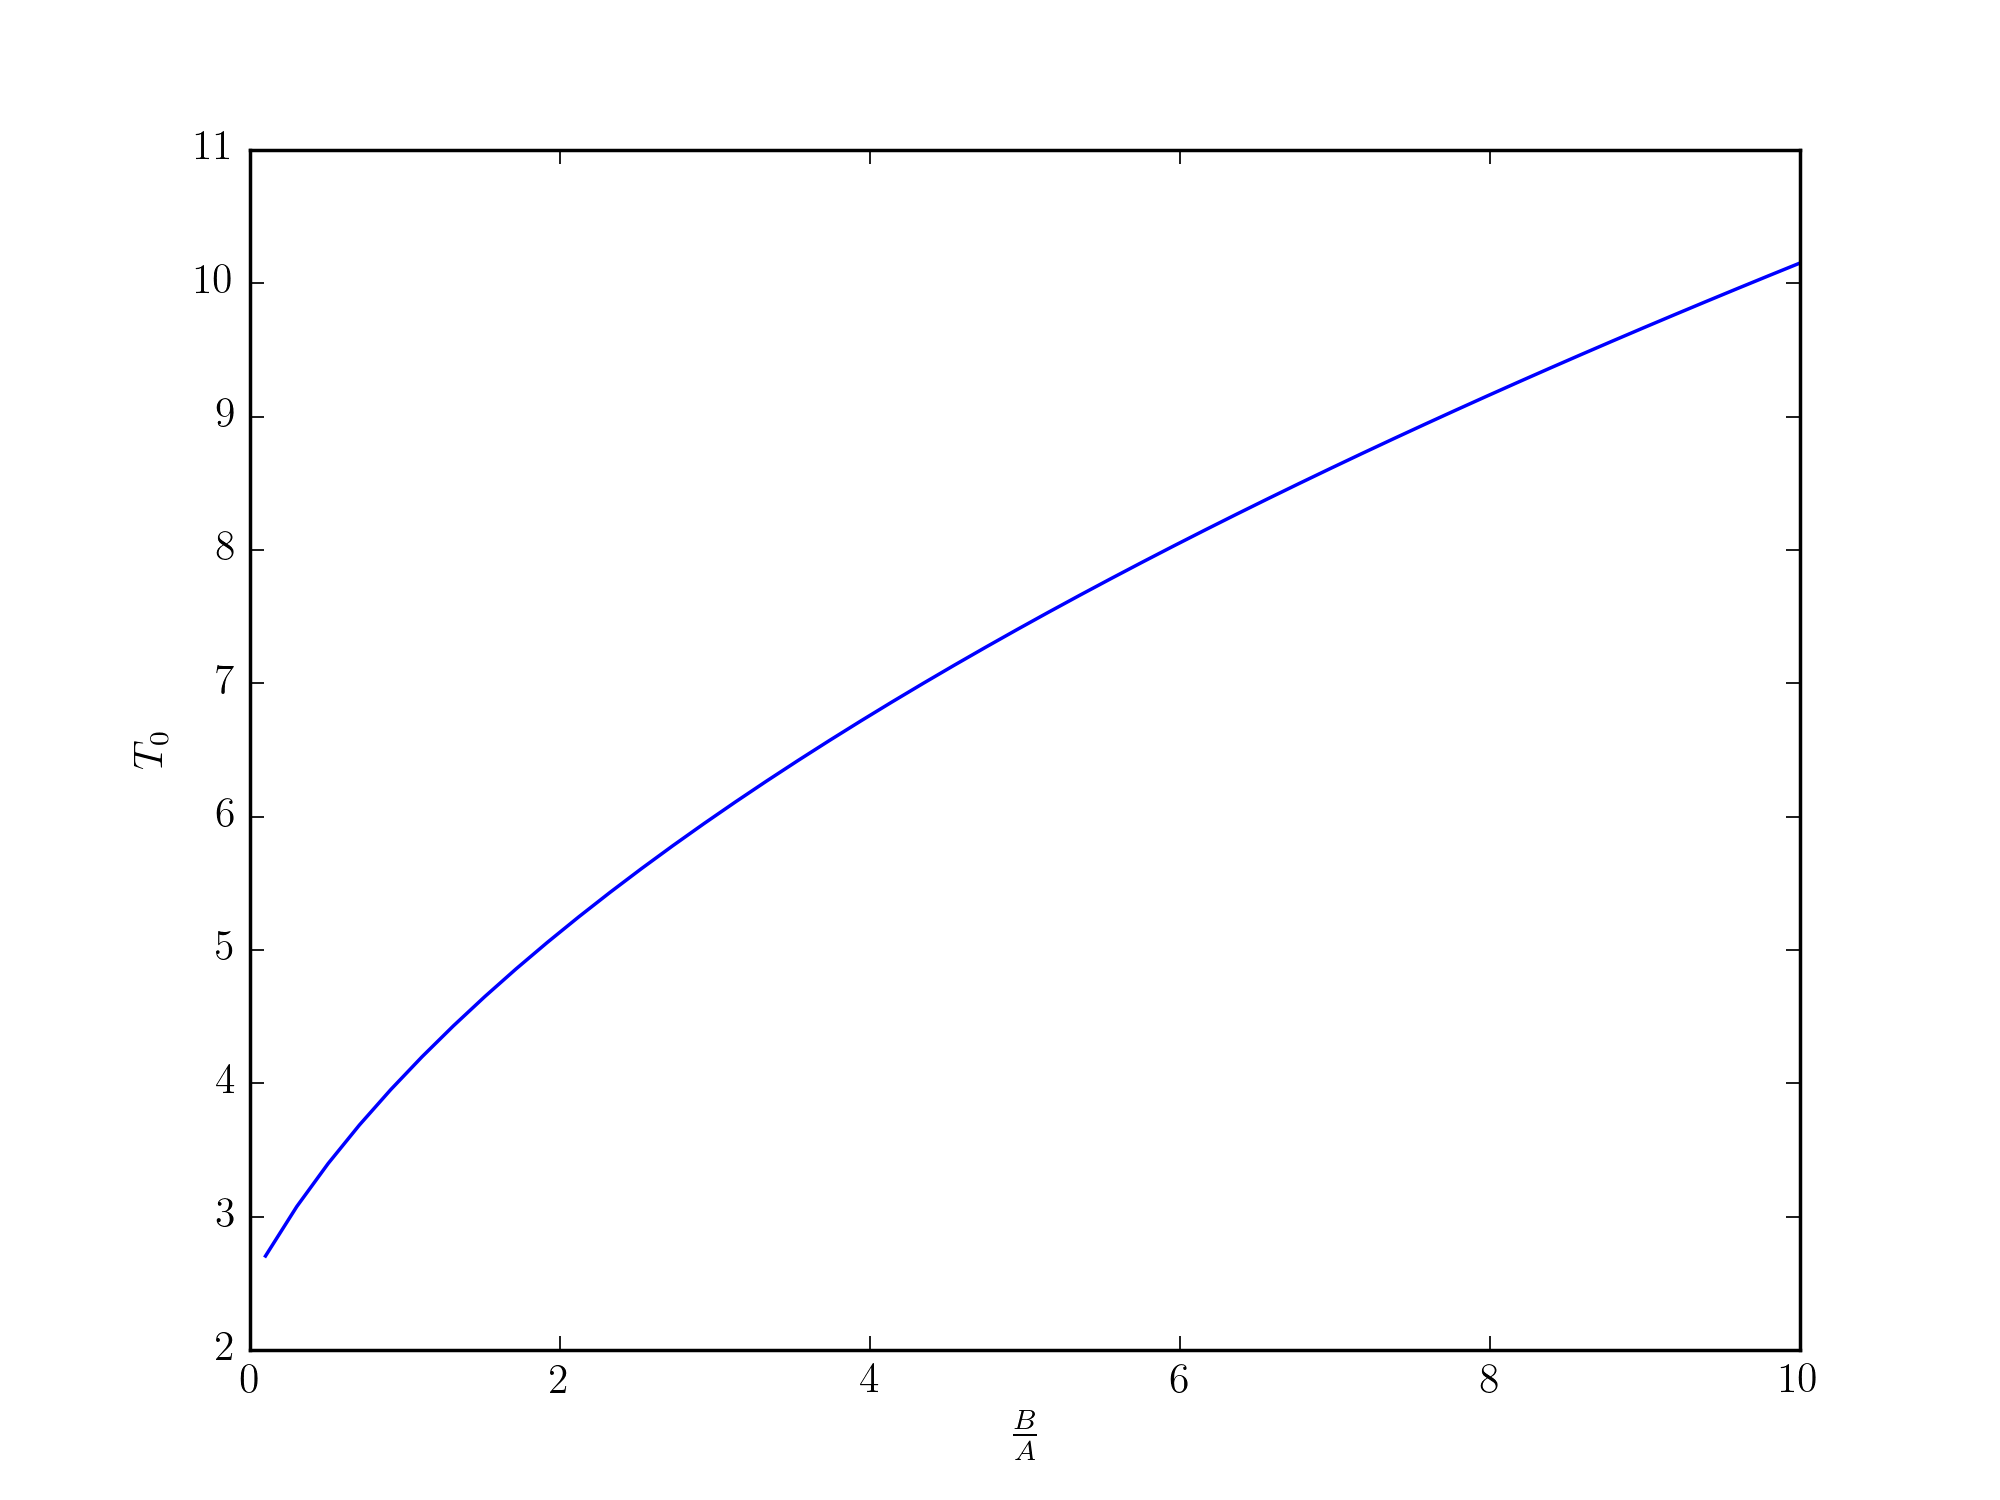
\includegraphics[width=0.7\textwidth]{figures/fig1.png}
\end{figure}

\newpage
\thispagestyle{empty}
\textbf{Solution}
\begin{enumerate}
  \item
    Conservation of energy states that the initial energy is equal to final energy, or any energy in between. The initial energy is:
    \begin{equation*}
      E_{i} = mgB
    \end{equation*}
    The energy at some height y is:
    \begin{equation*}
      E_{f} = mgy + \frac{1}{2}mv^2
    \end{equation*}
    Equating these and solving for $v^2$ yields:
    \begin{equation*}
      v^2=2g(B-y)
    \end{equation*}
  \item
    Substituting $v^2$ with $(\frac{dx}{dt})^2 + (\frac{dy}{dt})^2$ gives:
    \begin{align*}
      (\frac{dx}{dt})^2 + (\frac{dy}{dt})^2&=2g(B-y) \\
      \frac{ {dx}^2 +{dy}^2 }{ {dt}^2 } &=2g(B-y)    \\
      \frac{ {dx}^2 +{dy}^2 }{ 2g(B-y) } &={dt}^2    \\
      dt&=\sqrt{ \frac{ {dx}^2 +{dy}^2 }{ 2g(B-y) } }\\
    \end{align*}
  \item
    Factoring out a $dx$ gives:
    \begin{equation*}
      dt=\sqrt{ \frac{ 1 +(\frac{dy}{dx})^2 }{ 2g(B-y) } }dx
    \end{equation*}
    And replacing $\frac{dy}{dx}$ with the actual derivative gives
    \begin{equation*}
      dt=\sqrt{ \frac{ 1 +4\frac{x^2}{A^2} }{ 2g(B-\frac{x^2}{A}) } }dx
    \end{equation*}
  \item
    Integrating both sides gives:
    \begin{equation*}
      t = \int_{0}^{\sqrt{AB}}\sqrt{\frac{1+4\frac{x^2}{A^2}}{2g(B-\frac{x^2}{A}}}dx
    \end{equation*}
    Make integration substitution $\alpha=\frac{x^2}{AB}$ to simplify the integral gives:
    \begin{equation*}
      t =\sqrt{\frac{A}{8g}} \int_{0}^{1}\sqrt{\frac{1+4\frac{B}{A}\alpha}{\alpha-\alpha^2}}dx
    \end{equation*}
    Call the remaining integral $T_0(\frac{B}{A})$.
    \begin{equation*}
      t =\sqrt{\frac{A}{8g}} {T_0}\left(\frac{B}{A}\right)
    \end{equation*}

  \item
    The figure shows that $T_0$ is an increasing function of $\frac{B}{A}$, higher $B$ yields a larger time with $A$ held constant. Therefore, starting at a larger height results in a longer sled ride! \Smiley

\end{enumerate}

\end{document}
